\chapter{Computational Methods}
\label{ch:compmethods}

\begin{chapterabstract}
The theoretical basis of \mc{} methods and their application to generating realisations of \td{} networks is reviewed.
There is a broad discussion of Metropolis \mc{} methods, before specific methods are covered in detail; namely the bond switching algorithm and hard particle \mc{} in conjunction with the Voronoi construction.
This discussion lays the groundwork for the extension of these methods and development of additional \mc{} algorithms in subsequent chapters.
\end{chapterabstract}

\section{General \mc{} Methods}
\label{sec:mc}

\mc{} methods are a class of computational algorithms designed to solve complex problems stochastically.
These normally fall into the broad categories of calculating integrals, sampling probability distributions and finding global minima of very high dimensional functions \-- tasks which are often incredibly hard to compute deterministically.
Since their initial development in the mid\--20\th{} century, such methods have become an invaluable tool for solving problems in the physical sciences.
\mc{} methods are used in this context for calculating thermodynamic averages of properties in equilibrium systems; finding the minima in potential energy surfaces of small molecules, glasses, crystals and biomolecules; as well as non\--equilibrium simulations such as growth of crystals and thin\--films \cite{Landau2014,Wales1999,Levi1997,Ratsch2003,Kob1999,Jensen1999}.
In this thesis these \mc{} methods  will be used in a variety of contexts: chapter \ref{ch:bilayers} simulates the growth of bilayer materials using  a random sequential growth algorithm; chapter \ref{ch:targetedopt} optimises a cost function to control network structure; chapter \ref{ch:generalnetworks} samples amorphous configurations of various system topologies; chapter \ref{ch:quasi2d} samples the phase space of hard particle assemblies and chapter \ref{ch:procrystals} finds solutions to the procrystalline problem, essentially via global optimisation.
Therefore, the general theory is presented here with specific details of two established methods: bond switching and hard particle \mc{} given in the following section.

\subsection{Statistical Mechanics}

The total energy of a system with a fixed number of particles, $\mathcal{N}$, is given by the Hamiltonian,
\begin{equation}
	\ham = \ken+\pen \,,
\end{equation}
where $\ken$ is the kinetic energy as a function of all particle momenta and $\pen$ is the potential energy as a function of all particle positions \cite{Frenkel2002}.
The positions and momenta comprise the phase space of the system.
At fixed volume, $\mathcal{V}$, and temperature, $T$, all the the essential thermodynamic information is then provided through the classical canonical partition function:
\begin{equation}
	Q = \frac{1}{h^{D\mathcal{N}}\mathcal{N}!}\int \dd\mathbf{p}\,\dd\mathbf{r}\,\exp{\left[-\ham/ \kb T\right]}\,,
\end{equation}
where $D$ is the number of spatial dimensions.
This can be factorised into kinetic and potential components as
\begin{equation}
	Q = \frac{1}{h^{D\mathcal{N}}\mathcal{N}!}\int \dd\mathbf{p}\,\exp{\left[-\ken/\kb T\right]} \int \dd\mathbf{r}\,\exp{\left[-\pen/\kb T\right]} \,,
\end{equation}
where
\begin{equation}
	Z = \int \dd\mathbf{r}\,\exp{\left[-\pen/\kb T\right]}
\end{equation}
is the configurational integral \cite{Allen2017}. 
As will be shown, in \mc{} simulations it is the energetic differences between configurations that are required, and so at constant temperature the kinetic component can be neglected and it is only the configurational integral that is of importance.
In this case the probability density of the system being in the configuration $\mathbf{r}$, denoted $\mathcal{P}\left(\mathbf{r}\right)$, is given by the Boltzmann distribution:
\begin{equation}
	\label{eq:boltzmann}
	\mathcal{P}\left(\mathbf{r}\right) = \frac{\exp{\left[-\pen/\kb T\right]}}{Z}\,.
\end{equation}
This allows the expectation value of an observable of the system, $\obs$, to be determined from:
\begin{equation}
	\label{eq:expectationobs}
	%\langle A \rangle = \frac{1}{Z}\int \dd\mathbf{r}\,\obs\exp{\left[-\pen/\kb T\right]} \,.
		\langle A \rangle = \int \dd\mathbf{r}\,\obs \mathcal{P}\left(\mathbf{r}\right) \,.
\end{equation} 
The expectation value is then the ratio of two $\mathcal{N}D$ dimensional integrals.
The next section shows how these can be evaluated by \mc{} sampling.

\subsection{Importance Sampling}

An integral of form \eqref{eq:expectationobs} can be evaluated numerically by a number of methods.
As an illustration, consider the simple example of a \td{} potential energy surface in figure \ref{fig:montecarloint}.
To calculate the expectation value of the potential energy one must evaluate the integral
\begin{equation}
	\langle \mathcal{U} \rangle = \int_{0}^{L_y}\int_{0}^{L_x} \dd x \dd y\, \mathcal{U}\left(x,y\right)\mathcal{P}\left(x,y\right)\,.
\end{equation}
One way to achieve this would be to use standard numerical methods such as the trapezium rule or Simpson's rule to calculate the potential energy over a regular grid of points, as in figure \ref{fig:montecarloint1}, weighting each according to the Boltzmann distribution.

An alternative would be to take a stochastic approach.
In the simplest implementation, a series of $S$ random sampling points, $\left(x_i,y_i\right)$, can be generated uniformly in the intervals $\left[0,L_x\right]$ and $\left[0,L_y\right]$, as in figure \ref{fig:montecarloint2}.
Weighting these according to the Boltzmann distribution and averaging gives an estimation to the integral:
\begin{equation}
	\langle \mathcal{U} \rangle = \frac{L_xL_y}{S}\sum_{i=1}^{S} \mathcal{U}\left(x_i,y_i\right)\mathcal{P}\left(x_i,y_i\right)\,,
\end{equation}
which converges to the exact value as $S\rightarrow\infty$.

However, both quadrature and \mc{} uniform sampling suffer from the same inefficiency.
As can be seen in both schemes, many of the sampling points fall in regions of phase space where the potential energy is high and hence the weighting probability distribution is very small at reasonable temperatures.
In effect, significant effort is spent calculating regions where the contribution to the total integral is negligible.
A better approach is therefore to generate a series of $S$ random sampling points, $\left(x_i,y_i\right)$, according to the distribution $\mathcal{P}\left(x,y\right)$, as in figure \ref{fig:montecarloint3}.
The expectation value of the observable can then be calculated using a simple average:
\begin{equation}
	\langle \mathcal{U} \rangle = \frac{1}{S}\sum_{i=1}^{S} \mathcal{U}\left(x_i,y_i\right)\,.
\end{equation}
This is known as importance sampling and is vastly more efficient when dealing with an aggressive probability distribution like the Boltzmann, where only a small proportion of the phase space is readily accessible.

\begin{figure}[btp]
     \centering
     
     \begin{subfigure}[b]{0.48\textwidth}
         \centering
         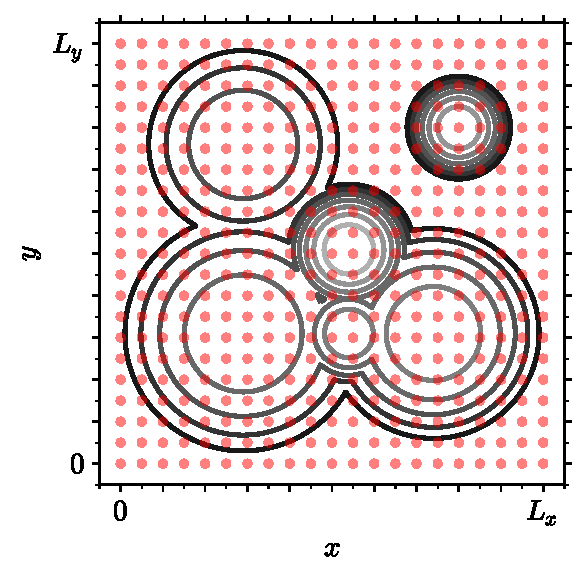
\includegraphics[width=\textwidth]{./figures/methods/mc_2d_quad.pdf}
         \caption{Quadrature}
         \label{fig:montecarloint1}
     \end{subfigure}
     \hfill
     \begin{subfigure}[b]{0.48\textwidth}
         \centering
         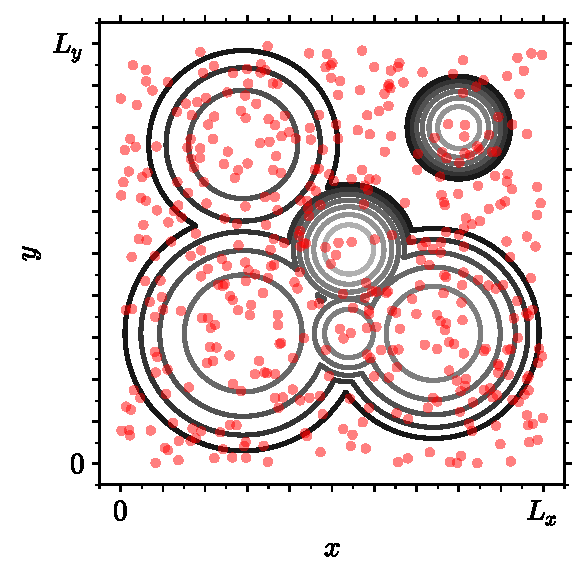
\includegraphics[width=\textwidth]{./figures/methods/mc_2d_rand.pdf}
         \caption{Uniform sampling}
         \label{fig:montecarloint2}
     \end{subfigure}
     \hfill
     
     \vspace{0.5cm}
     \begin{subfigure}[b]{0.48\textwidth}
         \centering
         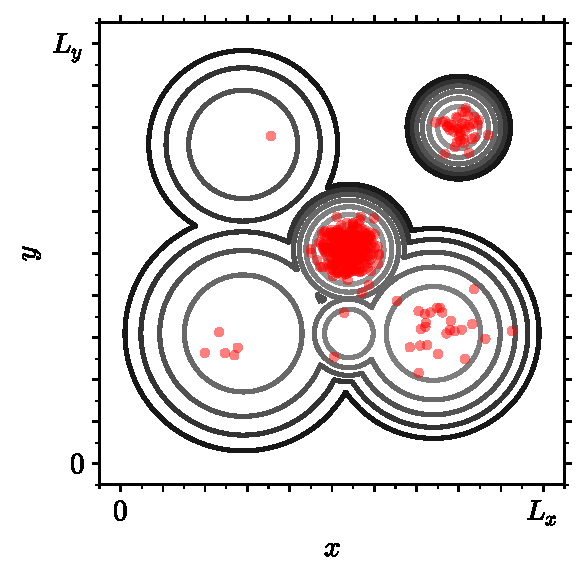
\includegraphics[width=\textwidth]{./figures/methods/mc_2d_imp.pdf}
         \caption{Importance sampling}
         \label{fig:montecarloint3}
     \end{subfigure}
     \hfill
     \begin{subfigure}[b]{0.48\textwidth}
         \centering
         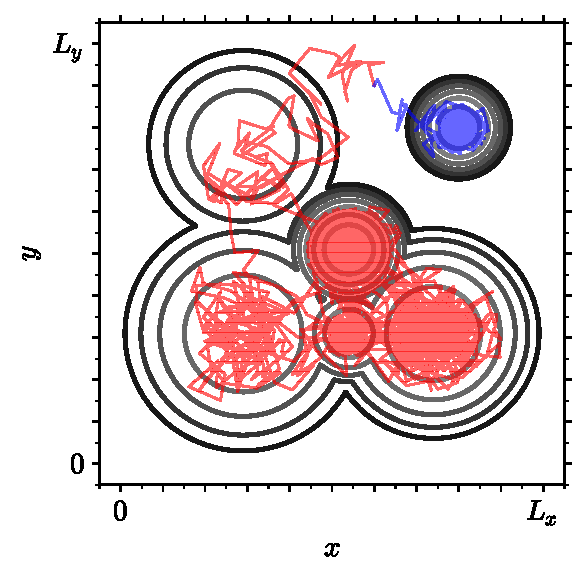
\includegraphics[width=\textwidth]{./figures/methods/mc_2d_mcmc.pdf}
         \caption{Markov Chain \mc}
         \label{fig:montecarloint4}
     \end{subfigure}
     \hfill
    
     \caption{Demonstration of different sampling methods with an example \td{} potential energy surface (contour lines). Panels (a)\--(c) display the same number of (red) sampling points. Panel (a) shows conventional quadrature where the surface is divided into a regular grid of sampling points which are then weighted by the Boltzmann distribution. Panel (b) shows \mc{} sampling with a uniform distribution of points which again must be Boltzmann\--weighted. Panel (c) shows \mc{} importance sampling with points now selected according to the Boltzmann distribution. Panel (d) shows Markov chain \mc{} with two random walks through phase space (red and blue lines) starting from different random seeds.}
     \label{fig:montecarloint}
\end{figure}

Whilst this scheme is ideal theoretically, it is impracticable for physical systems.
This is because for any problem of real interest one lives in a ``black box'' where the functional form of the potential energy surface in its hundreds if not thousands of dimensions is unknown.
In this case often the only way of learning about the form is by on\--the\--fly exploration of the surface \cite{Brooks2011}.
This can be achieved by talking a random walk through configurational space using Markov chain \mc.

\subsection{Markov Chain Monte Carlo}

Markov chain Monte Carlo provides a framework to perform importance sampling on a potential energy surface.
A system of interest can exist in a (very large) number of configurational states\footnote{In this work the notation $\vrc{i}$ will be used to denote all particle positions in a state $i$, whereas $\vrp{i}$ will be used to denote the $i$\th{} particle position in a given state.}, $\left\{\vrc{0},\vrc{1},\cdots,\vrc{M}\right\}$.
A Markov chain can then be constructed from this set, whereby a sequence of states is generated stochastically across a series of steps, $s=0,1,\dots,S$.
In this process, the probability of moving between states at each step is given by the transition matrix, $\bm{\pi}$, where each element, $\pi_{ij}$, gives the probability of moving from the state $\vrc{i}$ to another state $\vrc{j}$.  
This leads to the two relationships:
\begin{align}
	0\leq \pi_{ij} &\leq 1\,, \\
	\sum_{j} \pi_{ij} &= 1\,, \label{eq:tmrowsum}
\end{align}
the first being a statement of the probabilistic nature of the elements whilst the second ensures all transfer remains within the state space \cite{Frenkel2002,Allen2017,Brooks2011}.

The probability that the system is in each state at a given step, $s$, can be represented by the row vector $\mathbf{P}_s$.
This probability distribution evolves with each step as $\mathbf{P}_{s+1}=\mathbf{P}_{s}\bm{\pi}$, so that starting from any initial distribution, $\mathbf{P}_0$, it follows that $\mathbf{P}_S=\mathbf{P}_0\bm{\pi}^S$. 
The question is then as to the behaviour as $S\rightarrow \infty$.
Provided certain criteria are met, the distribution will tend to a stationary distribution, $\mathbf{P}$, which satisfies the eigenvalue equation 
\begin{equation}
	\mathbf{P} = \mathbf{P}\bm{\pi}\,, \label{eq:mcmceig}
\end{equation}
regardless of the initial distribution (although the speed of the convergence does depend on $\mathbf{P}_0$).
This will occur only if the system is \textit{ergodic}, meaning that every state is connected to every other by some finite path.

In a discrete analogue to equation \eqref{eq:expectationobs}, the expectation value of an observable, $A$, can be calculated from the ensemble average:
\begin{equation}
	\langle A \rangle = \sum_{i=1}^{M} A\left(\vrc{i}\right)\mathcal{P}\left(\vrc{i}\right)\,,
\end{equation}
where $\mathcal{P}\left(\vrc{i}\right)$ are the elements of $\mathbf{P}$.
However, as previously mentioned the number of discrete states is usually exceedingly large and so calculating the average over all states is not possible.
The solution is to take a random walk across through configurational space, sampling explicit states to form the chain $X_0,X_1,\dots,X_S$; where each move is chosen randomly according to the transition matrix $\bm{\pi}$.
In this case the expectation of the same observable can be calculated from the average over the sampled states:
\begin{equation}
	\langle A \rangle = \frac{1}{S}\sum_{i=1}^{S} A\left(X_i\right)\,,
\end{equation}
where the true value is approached as $S\rightarrow \infty$.

In this section the problem of sampling phase space efficiently has been reformulated, but as yet not solved. 
This is because the form of the transition matrix is still unknown.
Instead only the ideal form of the limiting probability distribution, $\mathbf{P}$, is available \-- where the elements follow the Boltzmann probabilities in equation \eqref{eq:boltzmann}.
A practical solution to this problem is provided by the Metropolis algorithm.

\subsection{Metropolis Algorithm}
\label{ssec:metropolis}

The Metropolis algorithm gives a prescription as to how to construct a transition matrix, $\bm{\pi}$, with the requisite properties, that samples the Boltzmann distribution \cite{Metropolis1953}.
Firstly, combining equations \eqref{eq:tmrowsum} and \eqref{eq:mcmceig} gives a condition on the transition matrix known as global balance:
\begin{equation}
	\sum_j \mathcal{P}\left(\vrc{i}\right)\pi_{ij} = \sum_j \mathcal{P}\left(\vrc{j}\right)\pi_{ji}\,.
\end{equation} 
Whilst it is possible to construct transition matrices which satisfy only global balance \cite{Manousiouthakis1999,Suwa2010,Michel2014}, it is practically simpler to satisfy global balance by applying the stronger condition of detailed balance:
\begin{equation}
	\mathcal{P}\left(\vrc{i}\right)\pi_{ij} = \mathcal{P}\left(\vrc{j}\right)\pi_{ji}\,.
\end{equation}
In the Metropolis algorithm the off\--diagonal elements of the transition matrix are written as the product of two probabilities: 
\begin{equation}
	\pi_{ij} = \begin{cases} 
		\tau_{ij}P_{ij} \quad & i\neq j \\
		1-\sum\limits_{j\neq i}\tau_{ij}P_{ij} \quad & i=j
	\end{cases}\,,
\end{equation}
where $\tau_{ij}$ is the trial probability of moving from state $\vrc{i}$ to $\vrc{j}$ and $P_{ij}$ is the probability of accepting the trial move.
To conform to detailed balance, the trial probabilities must be chosen to satisfy $\tau_{ij}=\tau_{ji}$.
Then, in the crux of the algorithm, the acceptance probabilities are given by
\begin{align}
	 P_{ij}&=\begin{cases}
	 	1 \quad &\mathcal{P}\left(\vrc{j}\right)\geq \mathcal{P}\left(\vrc{i}\right) \\
	 	\frac{\mathcal{P}\left(\vrc{j}\right)}{\mathcal{P}\left(\vrc{i}\right)} \quad & \mathcal{P}\left(\vrc{j}\right)< \mathcal{P}\left(\vrc{i}\right)
	 \end{cases}\,, \\
	 &=\begin{cases}
	 	1 \quad &\mathcal{U}\left(\vrc{j}\right)\leq \mathcal{U}\left(\vrc{i}\right) \\
	 	\frac{\exp\left[-\mathcal{U}\left(\vrc{j}\right)/\kb T\right]}{\exp\left[-\mathcal{U}\left(\vrc{i}\right)/\kb T\right]} \quad & \mathcal{U}\left(\vrc{j}\right)>\mathcal{U}\left(\vrc{i}\right)
	 \end{cases}\,,
\end{align}
which can be expressed more succinctly as
\begin{equation}
	\label{eq:metropolis}
	 P_{ij}=\text{min}\big[1,\exp\left[-\Delta \mathcal{U}/\kb T\right]\big]\,,
\end{equation}
where $\Delta \mathcal{U}$ is the difference in potential energy between the final and initial states.
The elegance of the Metropolis algorithm lies in the fact that the acceptance probability depends only on the ratio of the configuration probabilities removing the need for a normalising factor.
This means the relative probabilities can be used (which are computable) instead of the absolute probabilities (which are unknowable).

The final stage is the choice of the matrix of trial probabilities, $\bm{\tau}$. 
This is very flexible and one can be creative in the selection of trial moves, providing that the underlying matrix is symmetric and ergodic.
An effective strategy is to choose moves in which the trial state is relatively close to the current state to trace the paths of high probability in the system.
A summary of the Metropolis algorithm is therefore as follows:
\begin{enumerate}
	\item Initialise the system in a state $X_{s=0}$ and calculate the potential energy $\mathcal{U}\left(X_s\right)$
	\item Generate a trial state $X_t$ (a perturbation of $X_s$) according to $\tau_{st}$
	\item Calculate the potential energy of the trial state $\mathcal{U}\left(X_t\right)$
	\item Determine acceptance or rejection of the trial move according to the Metropolis criterion \eqref{eq:metropolis}
	\item Update the system to the new state: if the trial move is accepted $X_{s+1}=X_{t}$ otherwise $X_{s+1}=X_{s}$
	\item Repeat steps 2\--5
\end{enumerate}
There are a few practical factors related to the scheme above.
In Markov chain \mc{} it was previously mentioned that it takes time for the system to evolve to the stationary distribution.
Therefore it is necessary to have an equilibration period where the chain is generated but not used for sampling of observables.
In addition, whilst selecting trial moves close to the current state increases efficiency, it introduces correlation into the procedure.
A way around this is to not calculate observables based on every step, but rather after a number of statistically significant steps.

As an illustration of the Metropolis algorithm, consider again the \td{} potential energy surface in figure \ref{fig:montecarloint4}.
Here two simulation paths are displayed in red and blue, starting from the same initial state but with different %starting points in the random number generators \ie{} random seeds.
seeds in the random number generator.
As can be seen, the Metropolis algorithm takes a random walk over the configurational space, conducting importance sampling as in \ref{fig:montecarloint3}.
However, this example highlights a potential problem.
There are two regions of phase space with significant non\--zero probabilities which are separated by a relatively large energy barrier.
Although they are in principle linked by a path, the barrier may effectively mean they are disconnected with any reasonable number of steps, breaking ergodicity.
This manifests as the red walk sampling one region and the blue walk being trapped in the other region.
Using multiple seeds in this way helps to identify if any such behaviour is present.
If it leads to significant differences in the computed averages, more advanced techniques using enhanced sampling may have to be employed \cite{Torrie1977,Earl2005}.

\subsection{Global Optimisation and Simulated Annealing}
\label{s:simulatedannealing}

So far in this section, it has been shown how Monte Carlo methods can be used perform importance sampling of potential energy surfaces.
These methods can also be used to solve the related problem of finding global minima in potential energy surfaces and other more general functions.
Consider the case where there is an objective function, $\obj\left(\mathbf{r}\right)$, which depends on particle positions.
If it is known that there exists a solution where $\obj\left(\mathbf{r}\right)=0$, it may be sufficient to perform a standard random walk of the type in figure \ref{fig:montecarloint4} until a solution is found, using the more general Metropolis criterion:
\begin{equation}
	\label{eq:objmetropolis}
	P_{ij} = \min\big[1,\exp\left[-\Delta\Omega/\kb T\right]\big].
\end{equation}
There is of course a chance that the optimisation will not converge to the global minimum, most likely getting trapped in a local minimum (as for instance with the blue path in \ref{fig:montecarloint4}).
One solution to this problem is just to keep restarting the algorithm with different initial conditions until the global minimum is obtained.

Often however the value of the global minimum is not known, as is the case for a potential energy surface, and this rudimentary approach is insufficient.
One must then employ a more sophisticated technique to find the global minimum of a very high dimensional and potentially rough surface.
This in itself is an extensive area of study and there are many approaches, such as using genetic algorithms or basin\--hopping \cite{Hartke1993,Niesse1996,Wales1997}.
This thesis will use simulated annealing, which can be considered an extension to Metropolis \mc{} \cite{Kirkpatrick1983}.
In addition simulated annealing is effective for searching surfaces with many similar minima, as found in glasses.
Indeed, the name itself reflects its origins in the analogous metallurgical process to generate defect free metals.

\begin{figure}[tb]
     \centering
    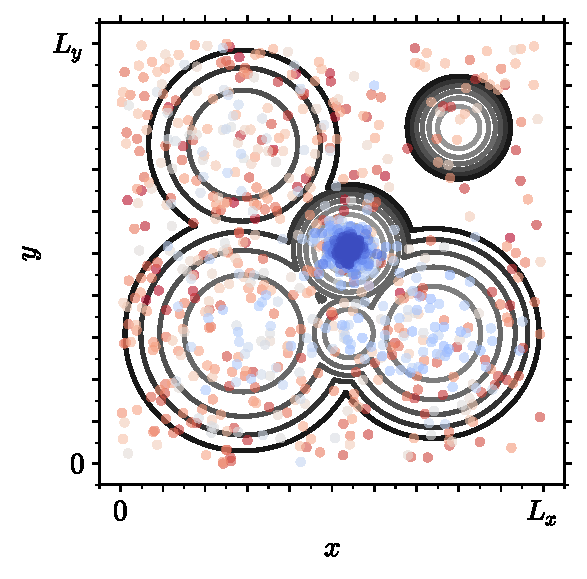
\includegraphics[width=0.48\textwidth]{./figures/methods/mc_2d_sa.pdf}
      \caption{Demonstration of the simulated annealing algorithm on a \td{} potential energy surface, with states coloured by temperature (red $\rightarrow$ blue indicating hot $\rightarrow$ cold. As the temperature is reduced the algorithm converges on the global minimum.}
      \label{fig:montecarloint5}
\end{figure}

The simulated annealing algorithm proceeds as follows.
The system of interest is first thermalised by performing Metropolis \mc{} at infinite temperature \ie{} accepting every move. 
The system is then gradually cooled to zero temperature, with the Metropolis criterion \eqref{eq:objmetropolis} reducing the proportion of accepted moves.
In theory if the cooling is infinitely slow, the system is maintained in thermal equilibrium and will eventually reach the global minimum \cite{Henderson2003}.
In practice this is not realisable and so a cooling rate must be empirically selected.
It is then still possible for trapping to occur in local minima, especially if the transition between low energy states is very slow.
As before, one can then cycle the simulated annealing, repeatedly heating and cooling the system until the global minimum is found.
The simulated annealing algorithm is demonstrated with the \td{} potential energy surface in figure \ref{fig:montecarloint5}.
Here, at high temperature the entire surface is sampled, overcoming all energy barriers, but as cooling takes place the system settles into the low energy regions of the surface, finally terminating in the global minimum.

\section{Bond Switching Monte Carlo}
\label{s:bondswitch}

Bond switching Monte Carlo was originally developed by Wooten, Winer and Weaire to generate high quality configurations of \thd{} silica glass \cite{Wooten1985}.
The basic principle is to amorphise a crystalline lattice with a series of transformations that swap the nearest neighbours of pairs of atoms, optimise the resulting structure and so generate a continuous random network (CRN) which is well\--relaxed.
These CRN models replicate experimental observables with high accuracy (including bond length and angle distributions, radial distribution functions, electronic band gaps and Raman spectra) and have since been applied to alternative systems such as three\--dimensional amorphous carbon, binary glasses and biological polymers \cite{Treacy2012,Tu1998,Djordjevic1995,Mousseau2004,Huisman2008,Broedersz2014}.
However, the method can also be readily modified to study \td{} systems, as has been done for amorphous graphene and silica, and which forms the basis for much of the work in this thesis, particularly in chapters \ref{ch:targetedopt}, \ref{ch:generalnetworks} and \ref{ch:ph} \cite{Kumar2014,Jain2018}.
The basic algorithmic details are described in this section, with extensions given in sections \ref{s:targetedoptalg} and \ref{s:genbondswitching}.

\subsection{Algorithmic Details} 

The \td{} bond switching algorithm essentially follows the prescription of simulated annealing in section \ref{s:simulatedannealing}.
A skeleton algorithm structure is outlined below, followed by specific details \cite{Kumar2012}.
Visualisations are provided for reference in figure \ref{fig:bsmc}.

\begin{enumerate}
	\item Generate initial crystalline hexagonal lattice
	\item Thermalise the lattice with a large number of random moves 
	\item Sample configurations by annealing the system slowly at finite temperature, accepting moves according to the Metropolis criterion \eqref{eq:metropolis}
\end{enumerate}
\begin{figure}[bt]
     \centering
     
     \begin{subfigure}[b]{0.24\textwidth}
    \centering
         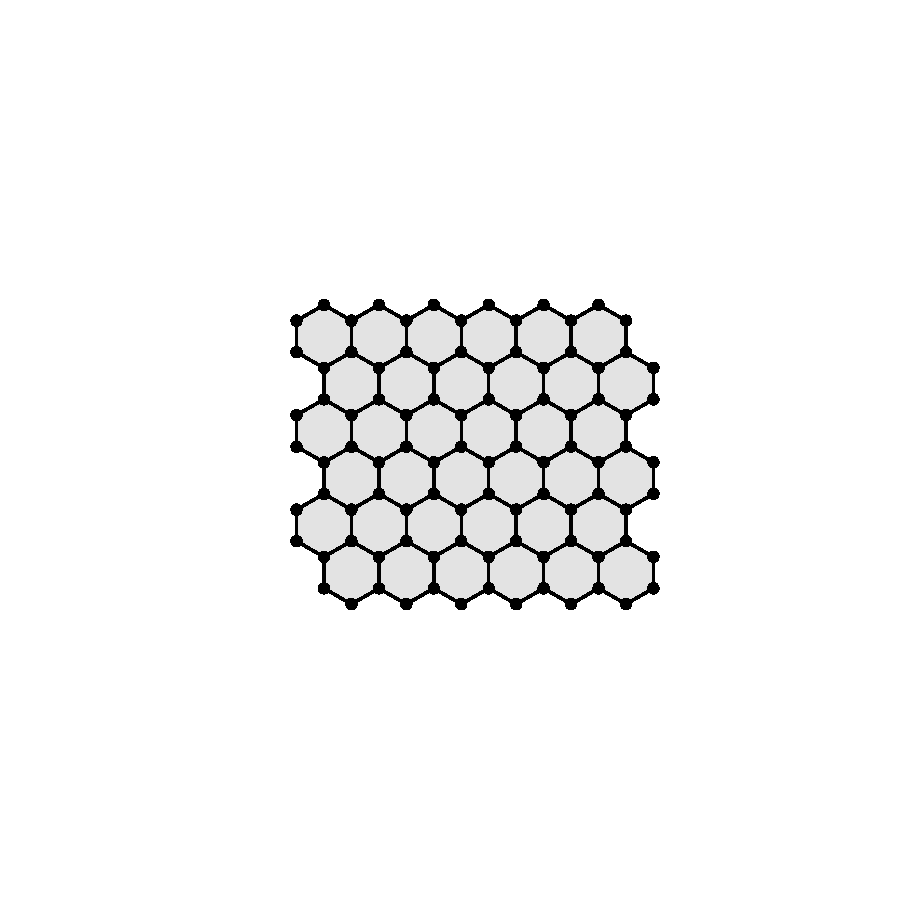
\includegraphics[height=2.8cm]{./figures/methods/bs_0.pdf}
         \caption{}
         \label{fig:bsmc1}
     \end{subfigure}
     \hfill
     \begin{subfigure}[b]{0.24\textwidth}
    \centering
         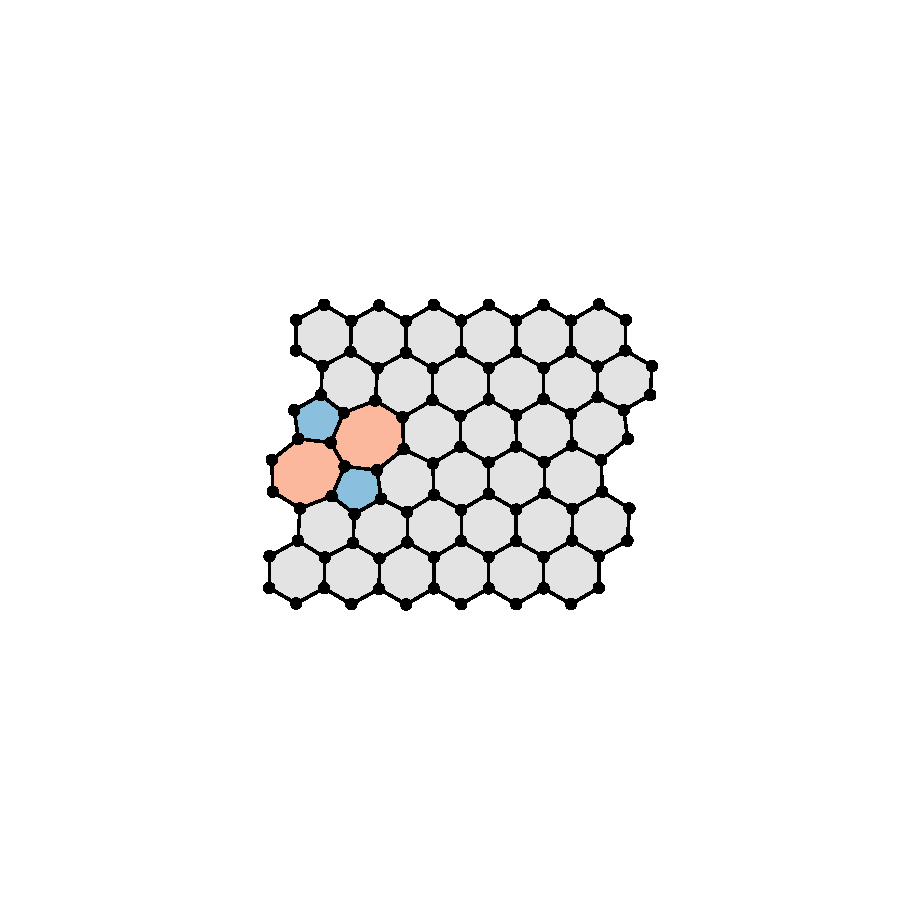
\includegraphics[height=2.8cm]{./figures/methods/bs_1.pdf}
         \caption{}
         \label{fig:bsmc2}
     \end{subfigure}
     \hfill
     \begin{subfigure}[b]{0.24\textwidth}
    \centering
         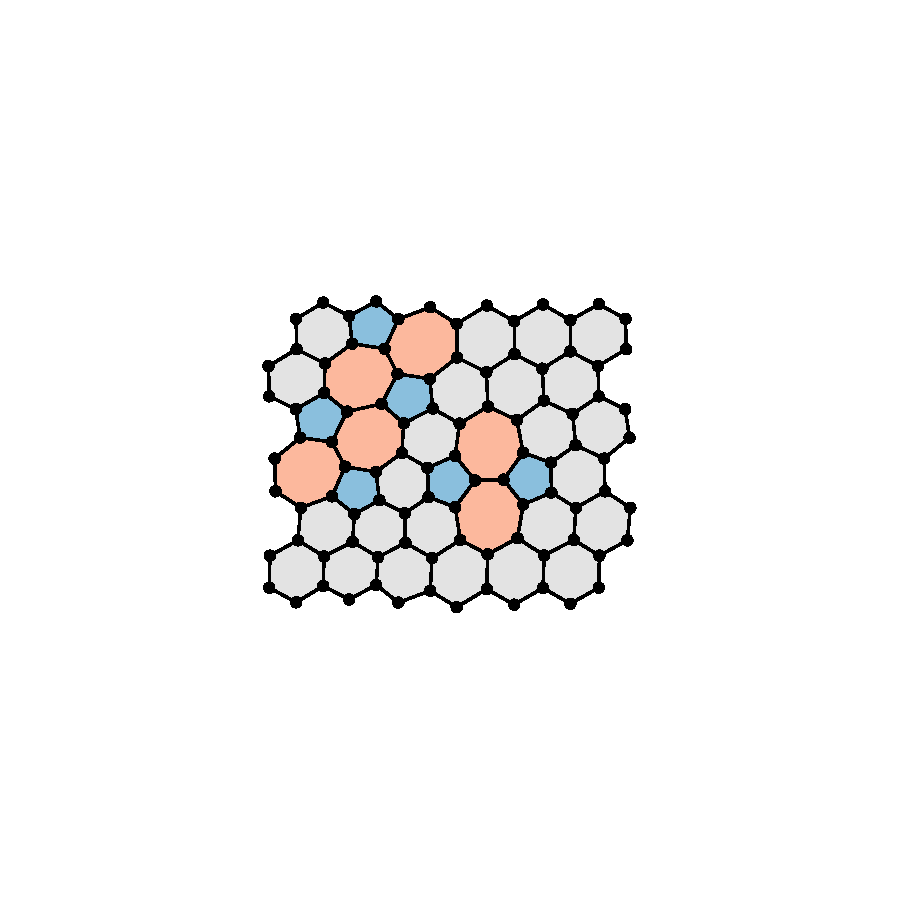
\includegraphics[height=2.8cm]{./figures/methods/bs_3.pdf}
         \caption{}
         \label{fig:bsmc3}
     \end{subfigure}
     \hfill
     \begin{subfigure}[b]{0.24\textwidth}
    \centering
         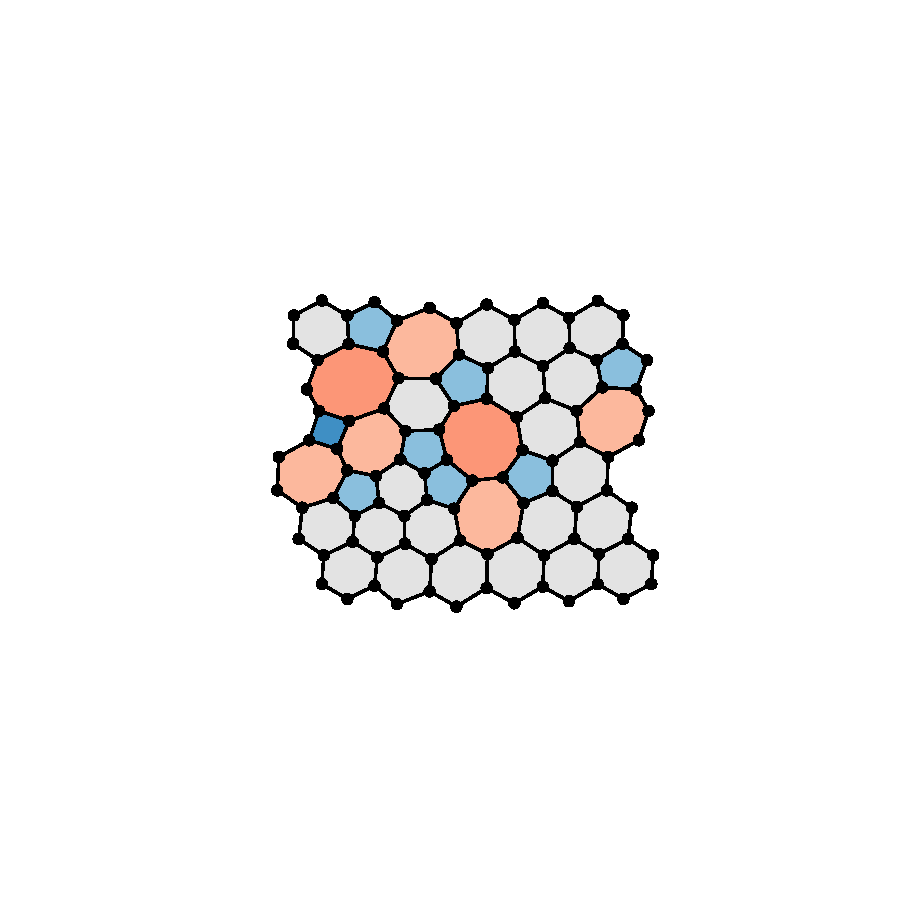
\includegraphics[height=2.8cm]{./figures/methods/bs_5.pdf}
         \caption{}
         \label{fig:bsmc4}
     \end{subfigure}
     
     \vspace{0.5cm}
     \begin{subfigure}[b]{0.24\textwidth}
     \centering
         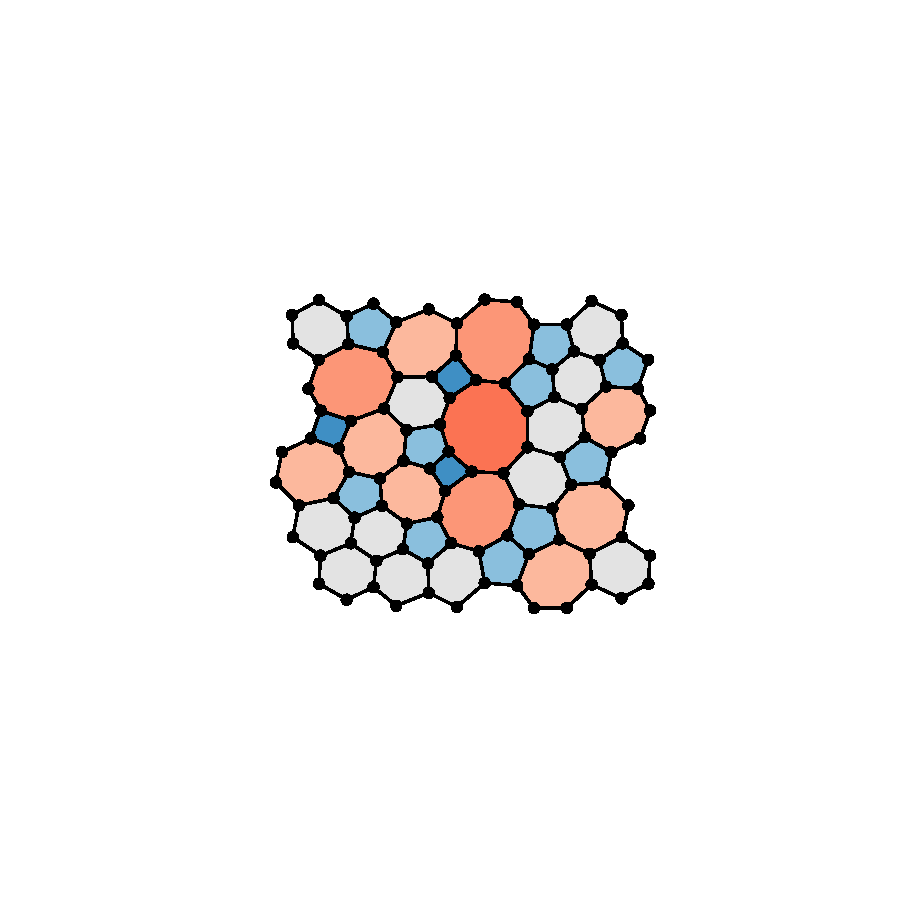
\includegraphics[height=2.8cm]{./figures/methods/bs_10.pdf}
         \caption{}
         \label{fig:bsmc5}
     \end{subfigure}
     \hfill
        \begin{subfigure}[b]{0.24\textwidth}
    \centering
         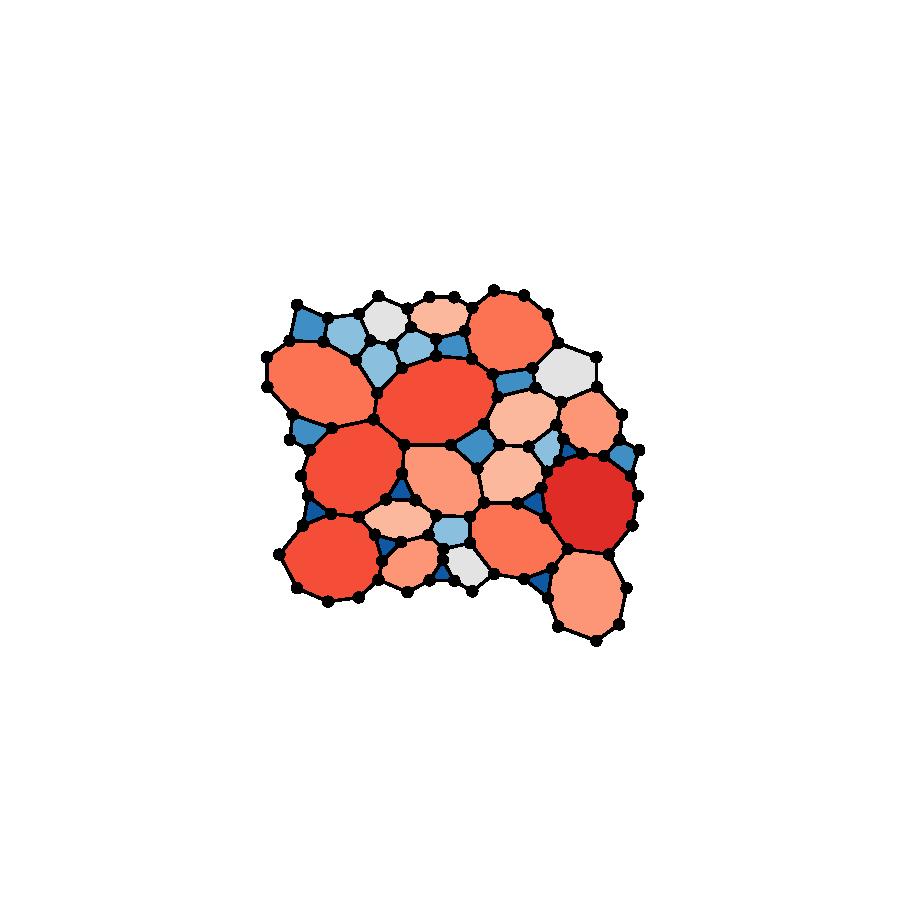
\includegraphics[height=2.8cm]{./figures/methods/bs_1000.pdf}
         \caption{}
         \label{fig:bsmc6}
     \end{subfigure}
     \hfill
           \begin{subfigure}[b]{0.24\textwidth}
    \centering
         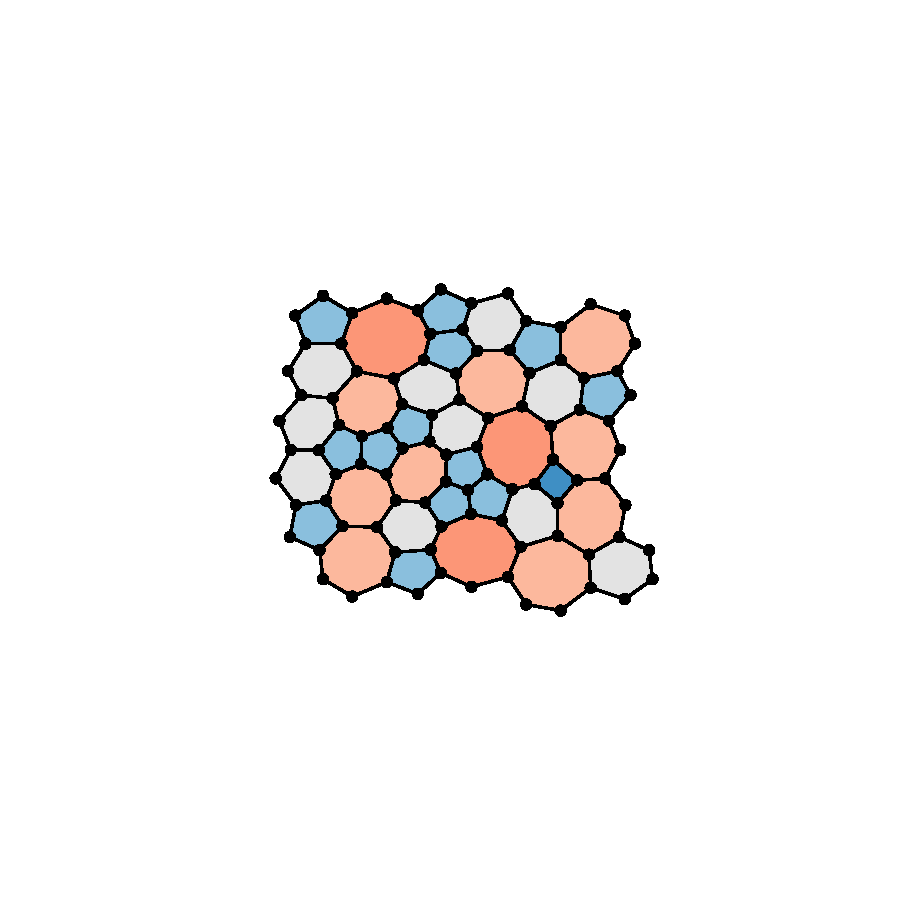
\includegraphics[height=2.8cm]{./figures/methods/bs_t1.pdf}
         \caption{}
         \label{fig:bsmc7}
     \end{subfigure}
     \hfill
           \begin{subfigure}[b]{0.24\textwidth}
    \centering
         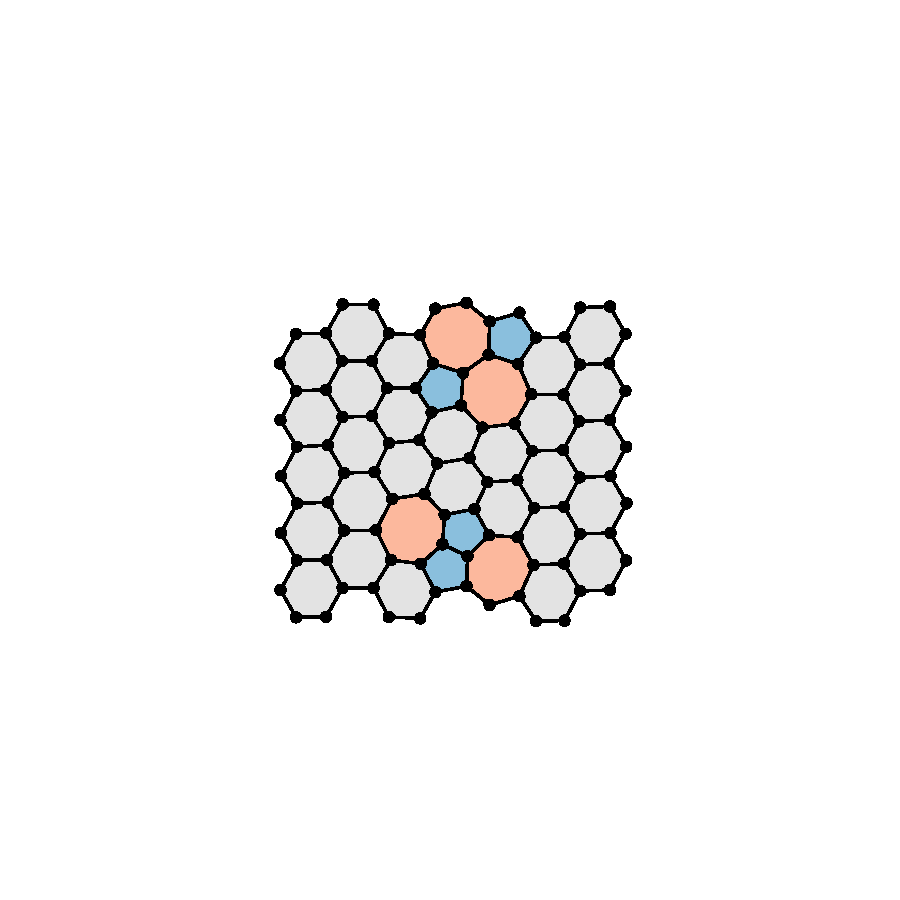
\includegraphics[height=2.8cm]{./figures/methods/bs_t2.pdf}
         \caption{}
         \label{fig:bsmc8}
     \end{subfigure}
   
     \caption{Configurations taken from stages of the \td{} bond switching algorithm. A crystalline lattice (a) is first thermalised to generate a random high energy network (f) by sequential overlapping Stone\--Wales defects (b)-(e). Sampling then occurs as the system is slowly annealed (g)-(h), allowing access to defect states that are not initially obtainable from the crystal structure.}
     \label{fig:bsmc}    
\end{figure}
The \mc{} move for 3\--coordinate atomic materials is essentially the introduction of a Stone\--Wales defect into the lattice, which
augments the size of two rings and decrements two others, preserving both the mean ring size and the coordination number of the individual atoms involved in the transformation \cite{Stone1986}.
As defects become more concentrated they overlap, leading to increasing diversity into the ring structure (allowing access to more than the pentagons and heptagons in a single Stone\--Wales defect).
Each bond transposition is followed by geometry optimisation to minimise and calculate the total energy of the system.  
A key aspect in the bond switching algorithm is therefore the choice of potential model.
The potential models and geometry optimisation process used in this thesis can be found in subsections \ref{s:potentials} and \ref{s:geomopt} below.

Cooling the system slowly ensures that the material remains in thermodynamic equilibrium, allowing configurations to be sampled throughout the simulation.
The ring structure of the system is then related to the temperature parameter, with more extreme ring sizes appearing at higher temperatures (compare figures \ref{fig:bsmc6}\--\ref{fig:bsmc8}).
This simply reflects the inherent balance of enthalpic \vs{} entropic  considerations.
Figure \ref{fig:bsmc8} also demonstrates the importance of cooling a randomised lattice instead of heating a crystal, as some low energy defects may have a multi\--step formation with a high energy barrier.  

\subsection{Potential Models}
\label{s:potentials}

To first address a matter of notation, in this thesis $\vrp{i}$ is used to denote the $i$\th{} particle position in a given configuration.
The vector between two particles is then defined $\vrp{ij}=\vrp{j}-\vrp{i}$.
The distance between two particles, $r_{ij}$, and the angle between three particles, $\theta_{ijk}$, are then given by:
\begin{align}
	r_{ij} &= \abs{\vrp{ij}}\,, \\
	\boldsymbol{\hat{\mathbf{r}}}_{ij} &= \frac{\vrp{ij}}{r_{ij}}\,, \\
	\boldsymbol{\hat{\mathbf{r}}}_{ij} \cdot \boldsymbol{\hat{\mathbf{r}}}_{ik}&=\cos\theta_{ijk}\,.
\end{align}
These will remain consistent throughout the work.

The nature of the bond switching method lends itself to the use of semi\--empirical potentials which have explicit stretching and angular neighbour lists.
As such a popular choice for materials modelling is the Keating potential and modifications thereof \cite{Keating1966,Barkema2000}. 
For a \td{} system the Keating potential has the form:
\begin{equation}
	\label{eq:keating}
	\pen = \frac{3}{16}\frac{\fk_S}{r_0^2}\sum_{\substack{i,j \in \\ \text{stretches}}} \left(r_{ij}^2-r_0^2\right)^2+
	\frac{3}{8}\frac{\fk_A}{r_0^2}\sum_{\substack{ijk \in \\ \text{angles}}}\left(r_{ij}r_{ik}\cos\theta_{ijk}-r_0^2\cos\theta_0\right)^2 \,,
\end{equation}
%where $r_{ij}$ the distance and $\theta_{ijk}$ the angle between particles; whilst 
where $\fk_S$ and $\fk_A$ are the force constants for the stretching and angular terms respectively \cite{Kumar2012}.
This potential drives the system towards equilibrium values of $r_0$ for the bond lengths and $\theta_0$ for the bond angles.
The Keating potential has been parametrised for a range of specific materials \cite{Kumar2012,Drabold2009}. 

However, a more generic potential model is sometimes required which captures the same essential physics.
This is provided through the simplified Keating potential \cite{VonAlfthan2003},
\begin{equation}
	\pen = \frac{\fk_S}{2}\sum_{\substack{i,j\in \\ \text{stretches}}}\left(r_{ij}-r_0\right)^2 + \frac{\fk_A}{2}\sum_{\substack{i,j,k \in \\ \text{angles}}} \left(\cos\theta_{ijk}-\cos\theta_0\right)^2\,,
\end{equation}
which is harmonic in stretching and angular terms.
A further modification can be made to this potential. 
Sometimes it is informative build models which enforce ring convexity \ie{} maintain all angles within the range $0\leq \theta_{ijk} \leq \pi$.
This can be achieved by augmenting the simplified Keating potential with a restricted bending (ReB) potential \cite{Bulacu2013}:
\begin{equation}
	\pen = \frac{\fk_S}{2}\sum_{\substack{i,j\in \\ \text{stretches}}}\left(r_{ij}-r_0\right)^2 + \frac{\fk_A}{2}\sum_{\substack{i,j,k \in \\ \text{angles}}} \frac{\left(\cos\theta_{ijk}-\cos\theta_0\right)^2}{\sin^{2}\theta_{ijk}}\,.
\end{equation}
The addition of the sine term in denominator causes the potential to diverge as bond angles approach linearity, preventing bonds from ``inverting''.

\subsection{Geometry Optimisation}
\label{s:geomopt}

The purpose of geometry optimisation is to minimise the overall potential energy of a network, $\pen$, as a function of all atomic positions, $\mathbf{r}$, after they have been perturbed \eg{} by a bond transposition.
As all initial configurations are well relaxed and perturbations relatively small, this can be achieved with a local minimisation routine.
In addition as the potential models in this work are smooth and harmonic, a straightforward steepest descent algorithm is both sufficient and efficient.

The steepest descent algorithm is an iterative method which searches down the potential energy gradient in a series of stages, $i$, until a minimum is reached \cite{Nocedal2006}.
It has the following scheme:
\begin{enumerate}
	\item Calculate the potential energy of the system $\mathcal{U}_i=\mathcal{U}\left(\mathbf{r}\right)$
	\item Determine the negative gradient of the potential \ie{} the forces acting on the particles $\mathbf{F}_i=-\nabla \mathcal{U}_i$ 
	\item Find the optimal distance to displace the particles along the lines of force $\mathcal{U}_{i+1}=\min \left[\mathcal{U}\left(\mathbf{r}+\lambda \mathbf{F}_i\right)\right]$
	\item Set $\mathbf{r}^{\prime}=\mathbf{r}+\lambda_{\text{min}} \mathbf{F}_i$
	\item Evaluate convergence and repeat steps 1-4 if $\left|\mathcal{U}_{i+1}-\mathcal{U}_i\right|>\kappa$
\end{enumerate}
The calculation of forces in stage 2 will depend on the potential model used, details of which are given in appendix \ref{app:forces}.
Note that stage 3 also requires a minimisation routine, which may seem counter\--intuitive. 
However, this is a one\--dimensional minimisation which trivial to estimate with a line search method \davidnote{Todo: decide on if appendix needed}.
The tightness of the convergence condition is set through the parameter $\kappa$.

One final performance improvement arises from the fact that the \mc{} moves are inherently local.
Therefore geometry optimisation can be employed such that only the atoms in the immediate vicinity of the switching move need to be minimised to obtain an accurate structure.
Typically this would extend to all atoms within five coordination shells of those directly involved in the switch move \cite{Mousseau2001}.

\section{Hard Particle \mc}
\label{s:hardparticlemc}

Hard particle Monte Carlo is one of the most well\--established computational methods in statistical physics.
Through its simplicity it is able to provide insight into the fundamental behaviour of particle systems and simulations of increasing size are still performed this century \cite{Isobe2016,Bernard2009,Anderson2013,Isobe2015}.
In this thesis it will be used to generate ring systems in the form of Voronoi tessellations (see section \ref{s:voronoiintro}), in analogy to experimental colloidal systems \cite{Thorneywork2017}.

\subsection{Hard Particle Model}
\label{s:hardparticlemodelintro}

Hard particle models are applicable over a range of dimensions.
In two dimensions the system consists of an arrangement of hard disks and in three dimensions hard spheres.
One can also take a quasi \td{} system, which comprises hard spheres confined to a plane.
Regardless of the dimensionality, the central principle is that no two particles in the system can have any degree overlap.
Formally, if the particle radii are denoted by $R_i$ and the distance between any pair of particle centres by $r_{ij}$, the pair potential is:
\begin{equation}
	\mathcal{U}_{ij} = \begin{cases}
	\infty \quad &r_{ij}<R_i+R_j \\
	0 \quad &\text{otherwise} %r_{ij}\geq R_i+R_j 
	\end{cases} \,.
\end{equation}
As the total energy is simply then
\begin{equation}
	\pen = \sum_{i<j} \mathcal{U}_{ij}\,,
\end{equation}
and it follows that if any pair of particles have overlap the system energy is infinite and the Boltzmann weighting is zero.
Hard particle models are typically quantified in terms of the packing fraction, $\phi$, which in two dimensions has the form
\begin{equation}
	\label{eq:packingfraction}
	\phi_{2D} = \rho\pi\langle R^2\rangle\,,
\end{equation}
where $\rho=\mathcal{N}/{V}$, the number density.

\subsection{Algorithmic Details} 

\begin{figure}[bt]
     \centering
     
     \begin{subfigure}[b]{0.25\textwidth}
         \centering
         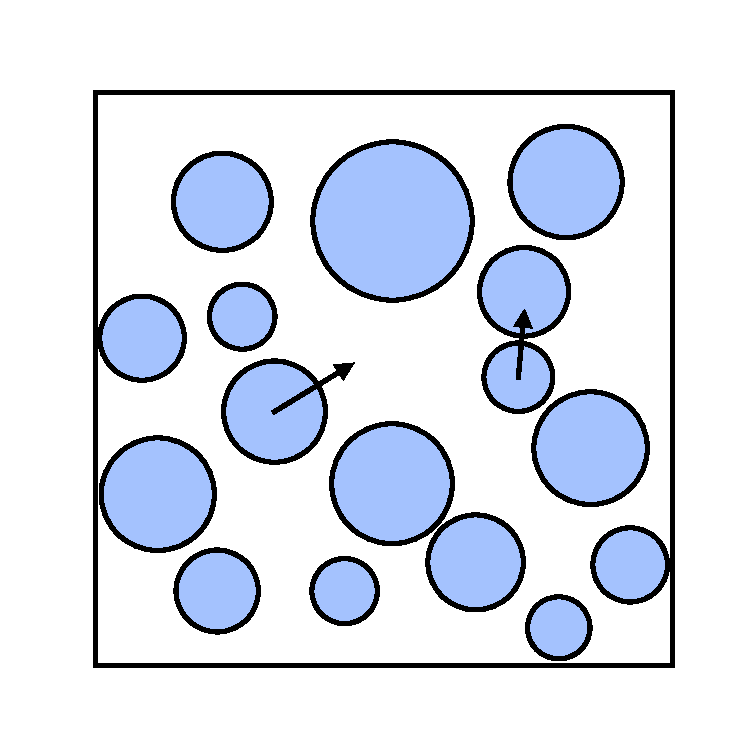
\includegraphics[width=3cm]{./figures/methods/mc_move_a.pdf}
         \caption{}
         \label{fig:hardmc1}
     \end{subfigure}
     \begin{subfigure}[b]{0.25\textwidth}
         \centering
         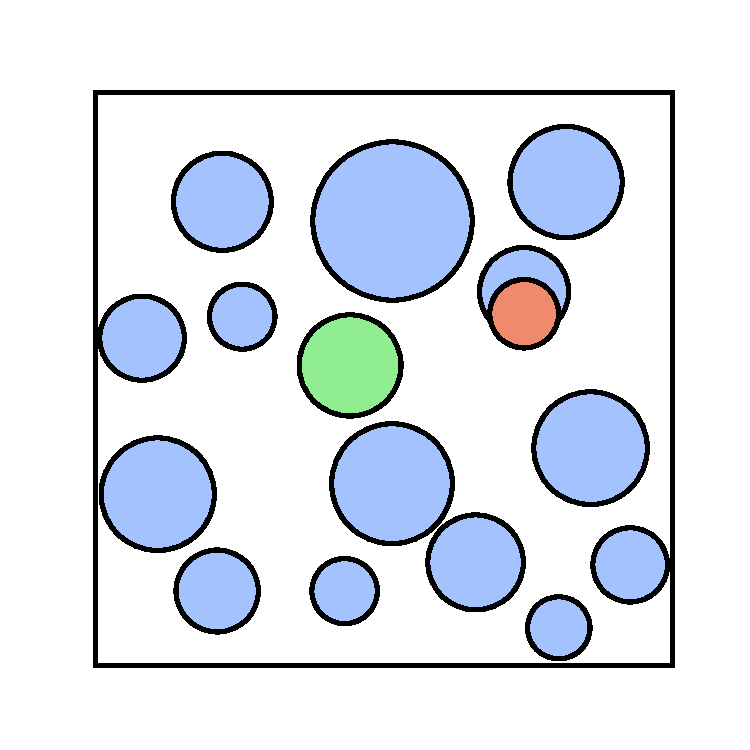
\includegraphics[width=3cm]{./figures/methods/mc_move_b.pdf}
         \caption{}
         \label{fig:hardmc2}
     \end{subfigure}
     \begin{subfigure}[b]{0.25\textwidth}
         \centering
         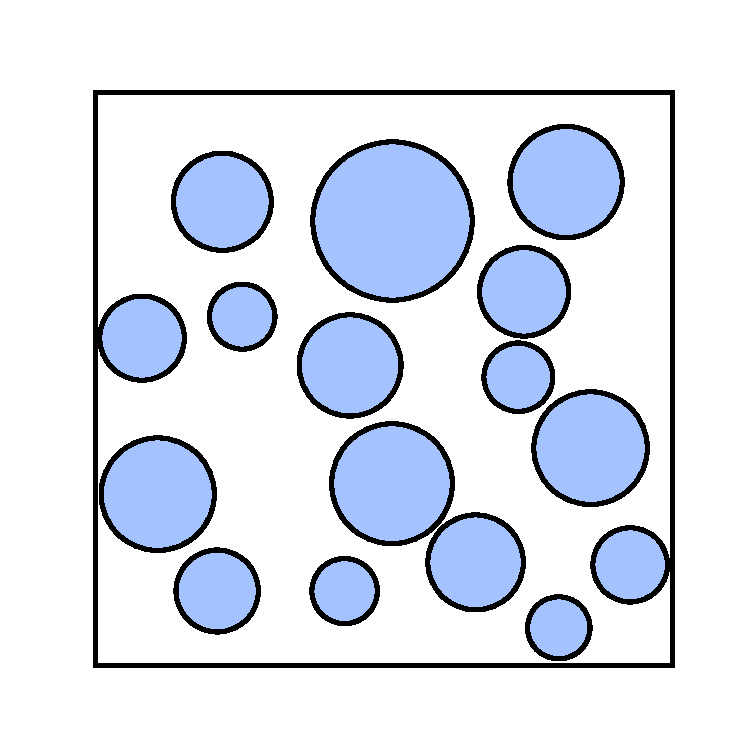
\includegraphics[width=3cm]{./figures/methods/mc_move_c.pdf}
         \caption{}
         \label{fig:hardmc3}
     \end{subfigure}
     
     	\vspace{0.5cm}
       \begin{subfigure}[b]{0.25\textwidth}
         \centering
         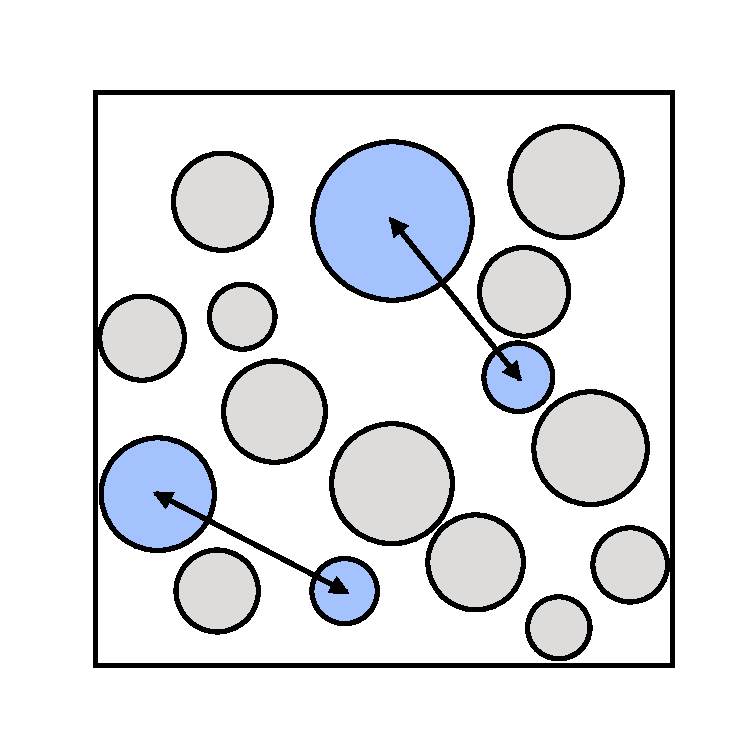
\includegraphics[width=3cm]{./figures/methods/mc_move_d.pdf}
         \caption{}
         \label{fig:hardmc4}
     \end{subfigure}
     \begin{subfigure}[b]{0.25\textwidth}
         \centering
         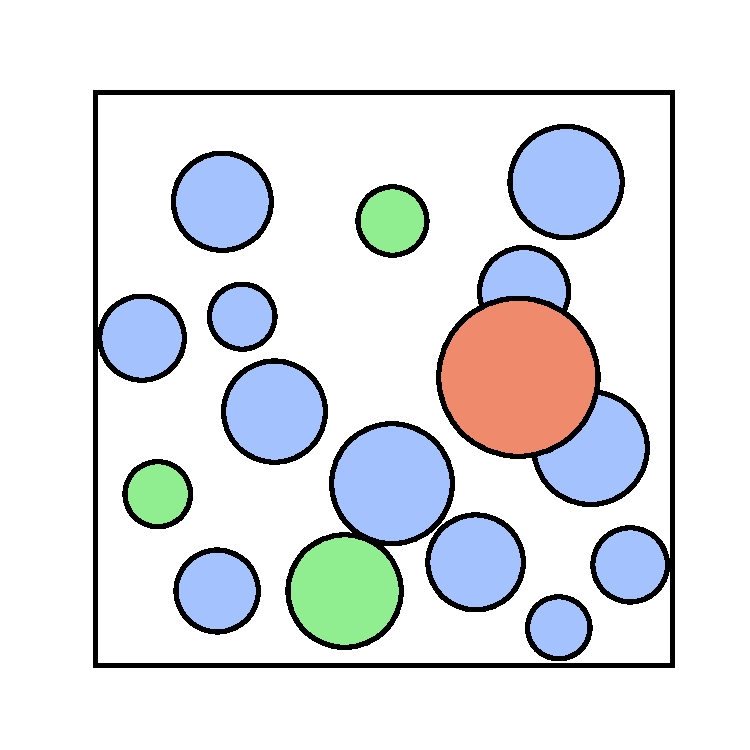
\includegraphics[width=3cm]{./figures/methods/mc_move_e.pdf}
         \caption{}
         \label{fig:hardmc5}
     \end{subfigure}
     \begin{subfigure}[b]{0.25\textwidth}
         \centering
         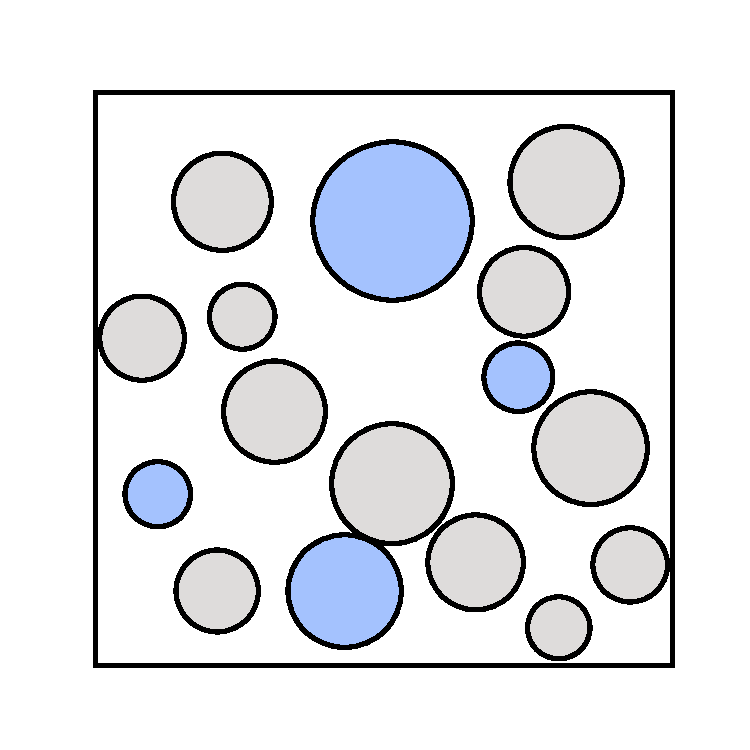
\includegraphics[width=3cm]{./figures/methods/mc_move_f.pdf}
         \caption{}
         \label{fig:hardmc6}
     \end{subfigure}
   
     \caption{Demonstration of two displacement (a)\--(c) and two swap (d)\--(f) moves in hard particle \mc.
     In displacement moves, particles are randomly selected and assigned a trial random displacement vector (a). In swap moves, two particles are randomly selected and as a trial their radii swapped (b). The trial move is then examined to see if it introduces any particle overlaps (b),(e). If there are no overlaps (green), then the trial move is accepted and the system updated but otherwise (red) the move is rejected and the system returns to the previous state (c),(f).
     }
     \label{fig:hardmc}
     
	\vspace{1cm}
	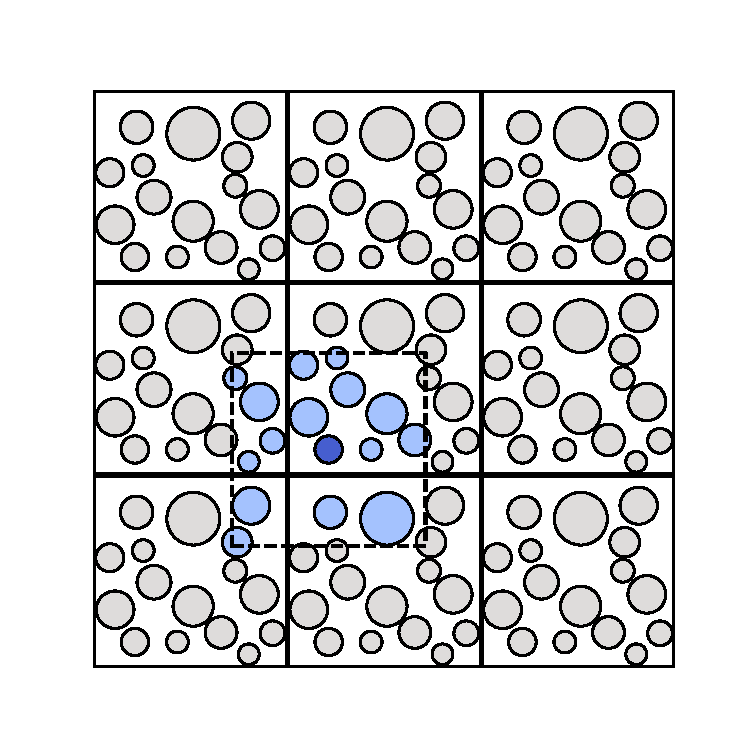
\includegraphics[width=5cm]{./figures/methods/mc_move_g.pdf}
	\caption{Simulation of bulk system is achieved using periodic boundary conditions, where a central cell is surrounded by repeated images of itself. A particle of interest (dark blue) then interacts with the nearest images of every other particle (light blue).}
	\label{fig:pbc}     
\end{figure}

Hard particle systems can be simulated using the Metropolis algorithm outlined in section \ref{ssec:metropolis}.
The system is initialised by selecting a random non\--overlapping configuration.
This can be achieved easily for low to medium densities by a greedy algorithm like random sequential addition, where particles are added successively in a manner which does not overlap with any previous particles \cite{Widom1966}.
For higher packing fractions a more sophisticated algorithm is needed where particles are swelled and their positions optimised \cite{Woodcock1976}.

Once the initial configuration has been generated, it is evolved via two \mc{} moves.
The first is the displacement move, whereby a random particle is selected and translated according to a random vector with elements generated uniformly in the range $\left[-\delta,\delta\right]$.
If the displacement introduces any particle overlaps it is rejected, otherwise the system is updated to the new configuration, as illustrated in figure \ref{fig:hardmc1}\--\ref{fig:hardmc3}.
The value of $\delta$ is chosen for each simulation such that the proportion of accepted moves is $\sim 50\%$, allowing for efficient searching of configurational space.
The optimal value can be determined by continuous adjustment during equilibration.

The second is the swap move, where two random particles are selected their radii exchanged \cite{Grigera2001,Ninarello2017}. 
Once again a swap move is only accepted if it does not lead to any overlapping particles and is demonstrated in figure \ref{fig:hardmc4}\--\ref{fig:hardmc6}.
The swap move is used to increase the efficiency in simulations of polydisperse particles and is an example of how the design of \mc{} moves can be flexible and that moves do not have to have a direct physical basis. 
The swap move is attempted for every ten displacement moves. 

Finally, to remove the presence of an interface in the system, simulation is performed with periodic boundary conditions.
In this scheme the central simulation cell is repeated to form an infinite lattice, so that every particle experiences a bulk environment.
Coupled with this is the use of the minimum image convention, where each particle then only interacts with the nearest repeated image of all the remaining particles.
This is illustrated in figure \ref{fig:pbc}.
 
\subsection{Voronoi Construction}
\label{s:voronoiintro}
\davidnote{Todo: could improve this, and construction diagram and paraboloid stuff}

The hard particle configurations produced by \mc{} simulations are not in themselves network structures, rather simply a collection of correlated points.
The network structure is revealed by construction of a Voronoi diagram, which partitions the sample into a system of tessellating cells, where each cell encapsulates all the space closest to the associated particle \cite{Okabe1992}.
Formally, given the set of particle positions $\mathbf{r}$, the Voronoi cell associated with a each particle, $V_i$, can be written
\begin{equation}
	V_i = \left\{\mathbf{x}\in {\rm I\!R}^D | \,\, \abs{\mathbf{x}-\vrp{i}}\leq \abs{\mathbf{x}-\vrp{j}} \,\, \forall \, i\neq j\right\}\,,
\end{equation}
so that the Voronoi diagram in its entirety is the set
\begin{equation}
	V = \left\{V_0, V_1, \cdots, V_\mathcal{N}\right\}\,.
\end{equation} 
More intuitively, a Voronoi diagram is formed through the placement of dividing lines between the centres of neighbouring particles. 
The intersection of these lines forms the characteristic tessellating polygons.

\begin{figure}[bt]
     \centering
     
     \begin{subfigure}[b]{0.22\textwidth}
         \centering
         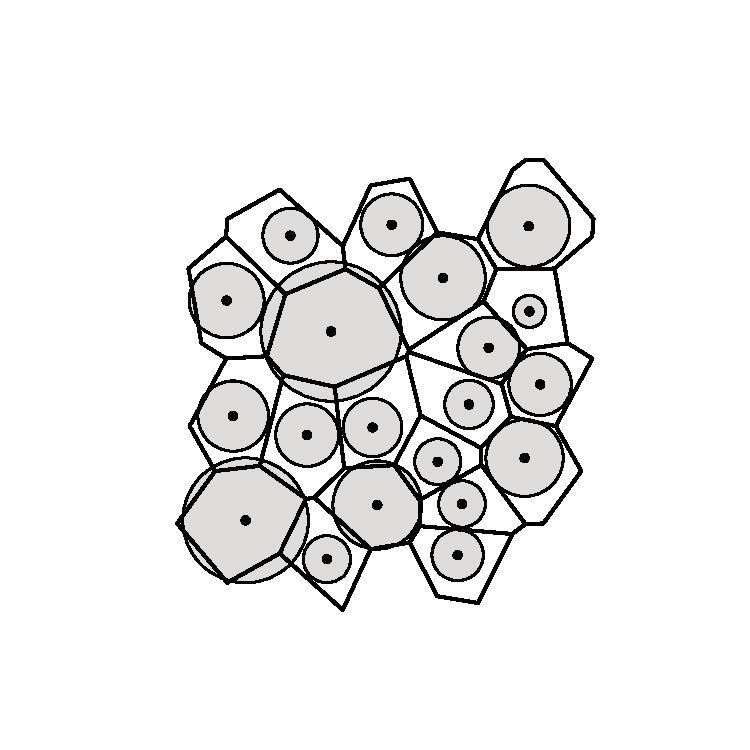
\includegraphics[width=\textwidth]{./figures/methods/voro_demo_vw.pdf}
         \caption{}
         \label{fig:vorodemov1}
     \end{subfigure}
     \hfill
     \begin{subfigure}[b]{0.22\textwidth}
         \centering
         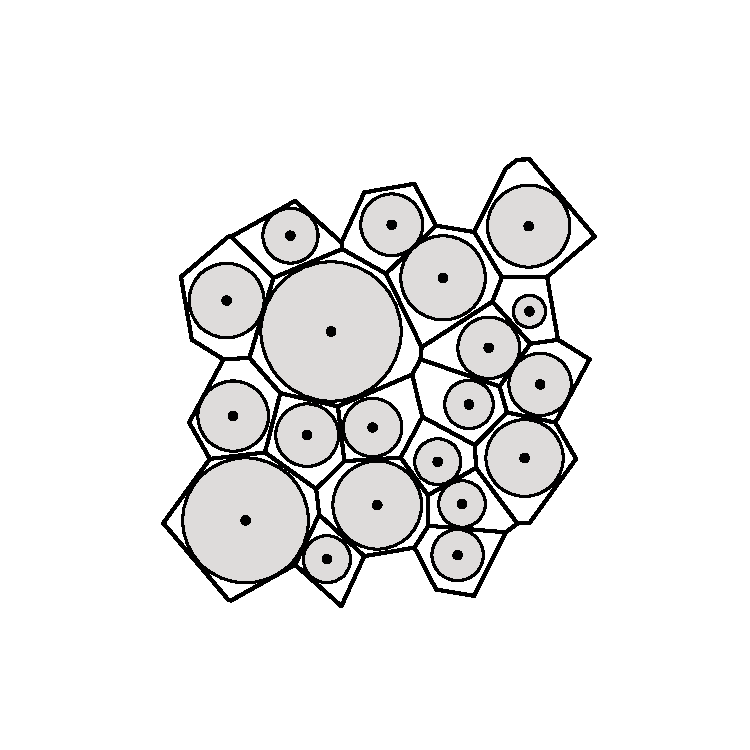
\includegraphics[width=\textwidth]{./figures/methods/voro_demo_rw.pdf}
         \caption{}
         \label{fig:vorodemor1}
     \end{subfigure}
     \hfill
     \begin{subfigure}[b]{0.22\textwidth}
         \centering
         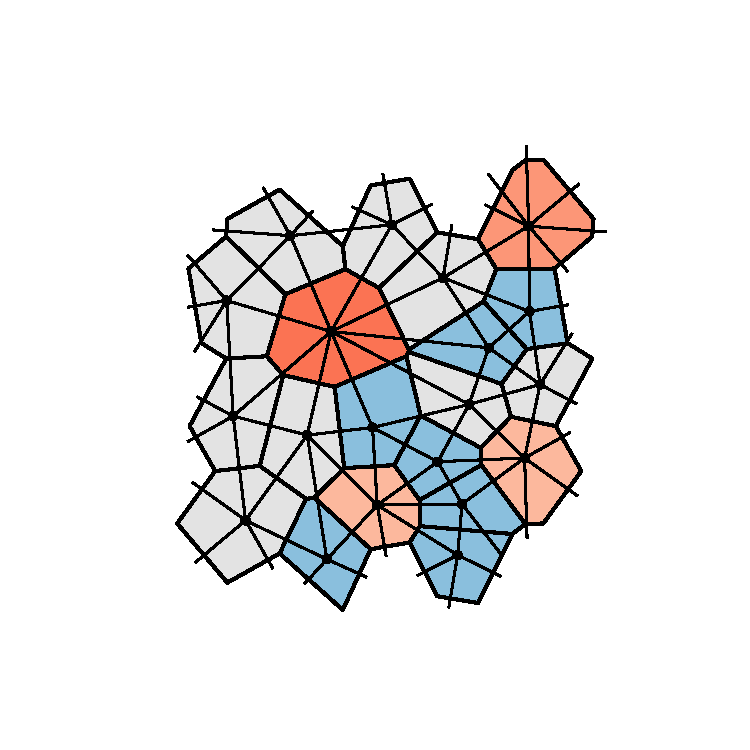
\includegraphics[width=\textwidth]{./figures/methods/voro_demo_vcd.pdf}
         \caption{}
         \label{fig:vorodemov2}
     \end{subfigure}
     \hfill
       \begin{subfigure}[b]{0.22\textwidth}
         \centering
         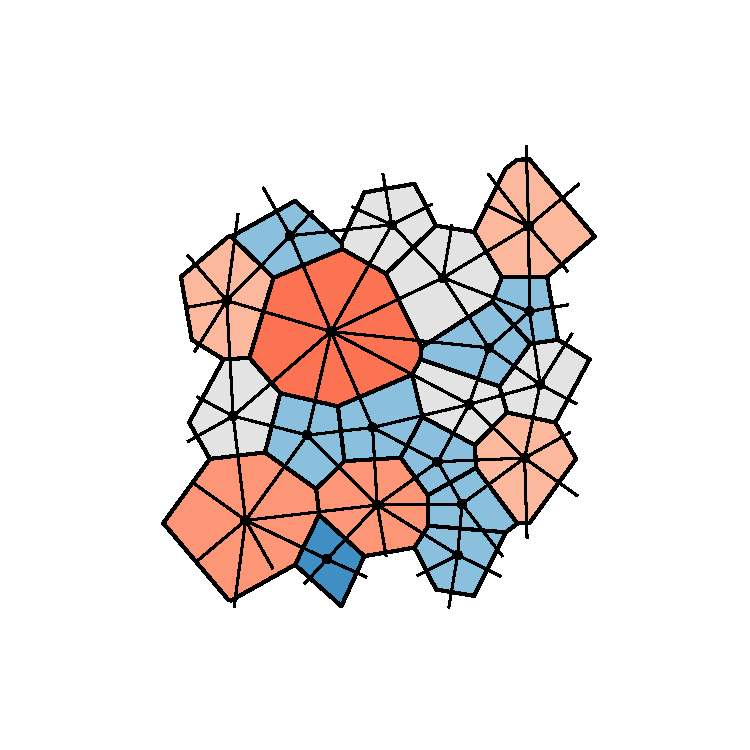
\includegraphics[width=\textwidth]{./figures/methods/voro_demo_rcd.pdf}
         \caption{}
         \label{fig:vorodemor2}
     \end{subfigure}
   
     \caption{Voronoi construction of a polydisperse hard disk system. Panels (a) and (b) compare the unweighted and weighted (radical) Voronoi tessellations respectively. The radical Voronoi assigns more volume to the larger particles to ensure a more equitable distribution of space, which can affect the underlying ring structure, shown in panels (c) and (d). The dual network, known as the Delaunay triangulation, is also overlaid.}
     \label{fig:vorodemo}
\end{figure}

In the simplest unweighted approach, the dividing line between two neighbouring particles separated by the Euclidean distance $r_{ij}$, is simply located midway between the particles at a distance $r_{ij} /2$. 
The elegance of the unweighted Voronoi diagram is that only the particle centres are required for its construction, with no requirement for a cut\--off parameter. 
Whilst the unweighted Voronoi tessellation is very effective for studying monodisperse particles, there are some limitations for polydisperse species. 
Specifically, the Voronoi partition underestimates the space assigned to large particles and overestimates that for small particles \-- a simple reflection of the lack of information on particle radii  (see figure \ref{fig:vorodemov1}). 
To rectify this, weighted modifications have been suggested which take account of the differences in radii \cite{Poupon2004}.

To construct a weighted Voronoi diagram, one simply adjusts the position of the dividing line, such that it is further from the particle with the greater weight. 
The weighting method used in this work is the so called radical tessellation, or power diagram \cite{GELLATLY1982,Aurenhammer1987}. In this modification, the dividing line is placed a distance $d_i$ from particle $i$, given by:
\begin{equation}
	\label{eq:radical}
	d_i = \frac{w_i^2-w_j^2+r_{ij}^2}{2r_{ij}}\,,
\end{equation}
where $w_i$ and $w_j$ are the weights for each particle. 
The benefit of this method is that is adjusts the partitioning of space so that greater volume is assigned to the particles with larger weight, and is well designed so that all of the sample space remains accounted for \-- unlike some alternative constructions \cite{Richards1974}. 
In terms of the particle weights, the logical choice is simply the particle radii. 
This is because at the contact distance, $r_{ij} = R_i + R_j$, equation \eqref{eq:radical} shows that $d_i = R_i$ \ie{} the radical dividing line sits exactly between the two particles, producing the most equitable distribution of volume (see figure \ref{fig:vorodemor1}). 
Furthermore, when the radii are equal, $d_i = r_{ij} /2$ and the result from the standard unweighted Voronoi is regenerated as expected.
It is worth noting here that the weighting method can affect the ring sizes (\ie{} number of vertices) as well as the ring areas, as demonstrated in figures \ref{fig:vorodemov2},\ref{fig:vorodemor2}.

The outcome of the Voronoi construction is a system of percolating rings not dissimilar to those seen in materials.
The dual network, known as the Delaunay triangulation, is also obtained, which defines the nearest neighbours for each particle.
The main difference with atomic materials is that the polygon edge lengths and angles are not constrained by a potential model the ring structure is therefore completely entropically controlled.
The degree of disorder is then determined by the packing fraction, $\phi$, where decreasing the packing fraction leads to increased diversity in the ring statistics, as illustrated in figure \ref{fig:voromono}.
As can be seen there are some defects which are analogous to those seen in materials, such as the Stone\--Wales defect in figure \ref{fig:voromono2}, but others are not, as in figure \ref{fig:voromono1} which arise from very small perturbations in the crystalline lattice.
The limiting value as $\phi\rightarrow 0$ is well studied as the Poisson Voronoi diagram \cite{Boots1983,Tanemura2003}.
This corresponds to the Voronoi diagram formed from a random uniform array of points.
In this way Voronoi systems provide a good complement to compare and contrast with materials.

\begin{figure}[bt]
     \centering
          \begin{subfigure}[b]{0.24\textwidth}
         \centering
         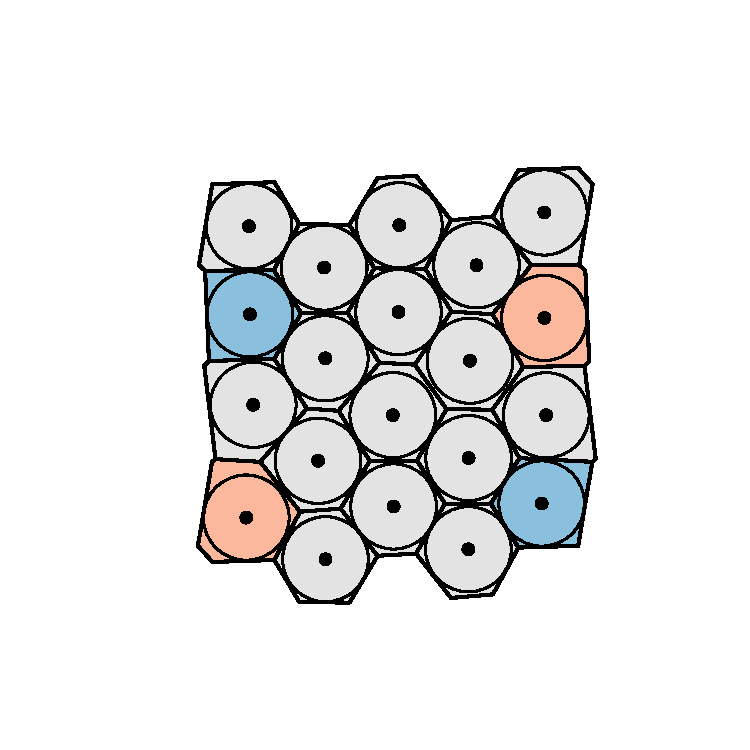
\includegraphics[height=3cm]{./figures/methods/voro_mono_80.pdf}
         \caption{$\phi=0.8$}
         \label{fig:voromono1}
     \end{subfigure}
     \hfill
     \begin{subfigure}[b]{0.24\textwidth}
         \centering
         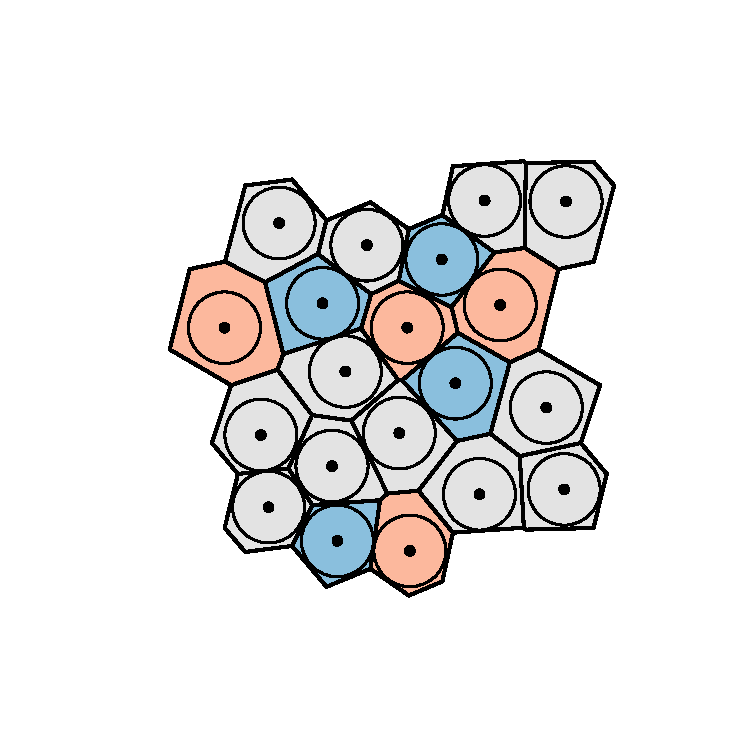
\includegraphics[height=3cm]{./figures/methods/voro_mono_60.pdf}
         \caption{$\phi=0.6$}
         \label{fig:voromono2}
     \end{subfigure}
     \hfill
     \begin{subfigure}[b]{0.24\textwidth}
         \centering
         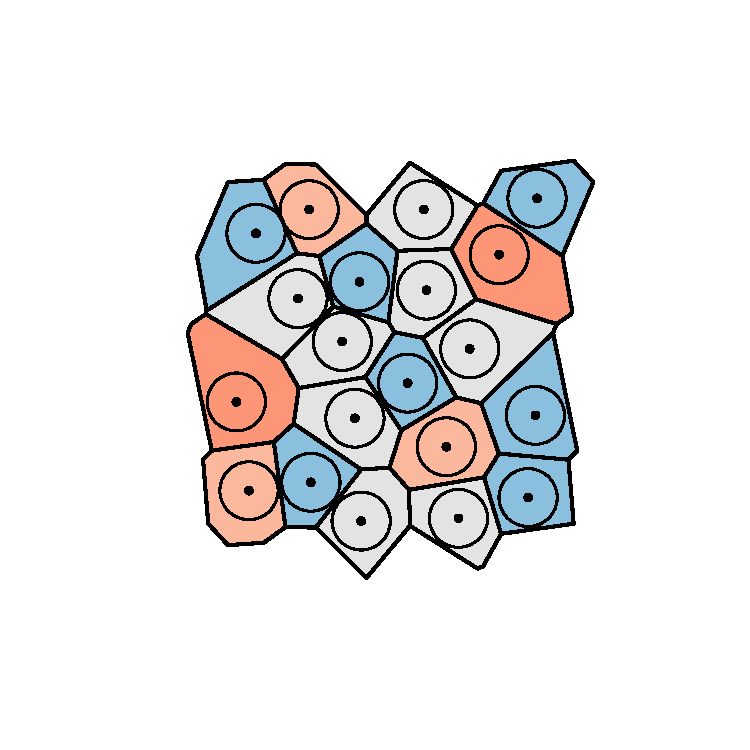
\includegraphics[height=3cm]{./figures/methods/voro_mono_40.pdf}
         \caption{$\phi=0.4$}
         \label{fig:voromono3}
     \end{subfigure}
     \hfill
       \begin{subfigure}[b]{0.24\textwidth}
         \centering
         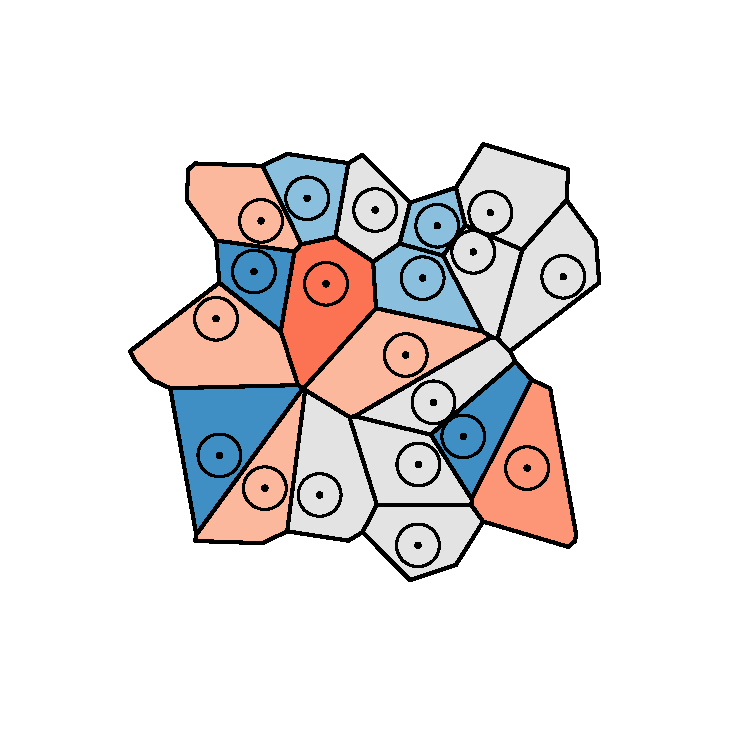
\includegraphics[height=3cm]{./figures/methods/voro_mono_20.pdf}
         \caption{$\phi=0.2$}
         \label{fig:voromono4}
     \end{subfigure}
     \caption{The ring structure in Voronoi diagrams is controlled through the packing fraction, $\phi$, of the underlying hard particle system. Ring diversity increases as packing fraction is lowered from $0.8\rightarrow 0.2$ in (a)\--(d).}
     \label{fig:voromono}
\end{figure}

In this thesis, the majority of Voronoi calculations were carried out practically using the excellent Voro\texttt{++} library \cite{Rycroft2009}.
\davidnote{Mention paraboloid stuff here???}

\section{Analysis Methods}

A wide variety of additional analysis methods are used throughout this thesis, to characterise configurations from simulation and experiment.
Most of these have either been covered in chapter \ref{ch:networktheory} or will be introduced as an accompaniment in relevant chapters, but more elementary techniques are established here.

\subsection{Bond Length and Angle Distributions}

The use of semi\--empirical potentials with precisely defined neighbour lists makes the evaluation of nearest\--neighbour bond lengths and angles straightforward.
The bond lengths, $r_{ij}$, can be calculated by scanning over all nearest\--neighbour pairs, whilst the angles, $\theta_{ijk}$, can equally be found by scanning over nearest\--neighbour triplets.
Histograms can then be constructed for each interaction type, denoted $f\left(r\right)$ and $f\left(\theta\right)$, for lengths and angles respectively.

\subsection{Radial Distribution Functions}

For a given point set, the radial distribution function (RDF or $g\left(r\right)$), gives the probability of finding a point at a distance $r$ from a reference point, normalised against a system of randomly distributed points at the same density.  
The RDF in two dimensions is then given by:
\begin{equation}
	g\left(r\right)=\frac{1}{2 \mathcal{N} \rho \pi r}\left\langle \sum_i \sum_{j\neq i} \delta\left(r-r_{ij}\right)\right\rangle\,. 
\end{equation} 
The behaviour of the RDF is therefore such that $g\left(r\right)>1$ indicates an increase in probability and $g\left(r\right)<1$ a corresponding decrease in probability, that two points are at a given separation relative to a random distribution.
For disordered media, any correlations inevitably decay with distance such that $\lim_{r\rightarrow \infty} g\left(r\right)=1$.

The reason this is framed in terms of generic point sets, is that in this thesis the RDF will be applied to the dual of the atomic coordinates, to measure ring\--ring spatial correlations.
Furthermore, partial RDFs will be employed, to measure correlations between rings of different sizes.
If these sizes are denoted, $a,b$, the partial RDF, $g_{ab}\left(r\right)$, is then given by:
\begin{equation}
	g_{ab}\left(r\right)=\frac{1}{2 \mathcal{N}_a \rho_b \pi r}\left\langle \sum_i \sum_{j\neq i} \delta\left(r-r_{ij}\right)\right\rangle\,, 
\end{equation} 
where $\mathcal{N}_a$ is the number of $a$\--rings and $\rho_b$ the density of $b$\--rings.
Hence the partial RDFs are normalised in a way to yield analogous behaviour to the total RDF.



